%Author: Steven Munn, Weiting Ling, Tianchen Jin
%UCSB ECE 278 Final write-up

%HEADERS
\documentclass[12pt, english, titlepage]{article}

\usepackage{seqsplit}
\usepackage{listings}
\usepackage[T1]{fontenc}
\usepackage[latin9]{inputenc}
\usepackage[letterpaper]{geometry}
\usepackage{wrapfig}
\usepackage{graphicx}
\usepackage{caption}
\usepackage{subcaption}
\usepackage{babel}
\usepackage{amstext}
\usepackage{amsmath}
\usepackage{hyperref}
\usepackage{units}
\usepackage{algorithmicx}
\usepackage{algpseudocode}
\usepackage{amssymb}
\usepackage[ampersand]{easylist}

\usepackage{listings}
\usepackage{color}

\definecolor{dkgreen}{rgb}{0,0.6,0}
\definecolor{gray}{rgb}{0.5,0.5,0.5}
\definecolor{mauve}{rgb}{0.58,0,0.82}

\ListProperties(Hide=100, Hang=true, Progressive=3ex, Style*=$\bullet$ ,
Style2*=$\Rightarrow$)
\lstset{frame=tb,
  language=matlab,
  aboveskip=3mm,
  belowskip=3mm,
  showstringspaces=false,
  columns=flexible,
  basicstyle={\small\ttfamily},
  numbers=none,
  numberstyle=\tiny\color{gray},
  keywordstyle=\color{blue},
  commentstyle=\color{dkgreen},
  stringstyle=\color{mauve},
  breaklines=true,
  breakatwhitespace=true
  tabsize=0
}

\geometry{verbose,tmargin=1in,bmargin=1in,lmargin=1in,rmargin=1in}

\setlength{\parskip}{\smallskipamount}
\setlength{\parindent}{0pt}
\setlength{\parindent}{0.25in}

\newcommand{\tab}{\hspace*{2em}}
%\newcommand{\unit}[1]{\ensuremath{\, \mathrm{#1}}}
\newcommand{\btheta}{\boldsymbol{\theta}}
\newcommand{\p}[1]{\left(#1\right)}
%END HEADERS

\begin{document}

\title{Efficient Graph-based Image Segmentation}

\author{TianChen Jin, Weiting Lin, Steven Munn}

\date{Friday, March 13, 2015}

\maketitle

\section{Questions}

\begin{enumerate}
\item In 2-3 sentences, describe the main project goal.

Our project implements \emph{Efficient Graph-based segmentation} by Felzenszwalb \ref{paper}, first in C/C++, then as a mex wrapper for use with MATLAB, and finally, in Android for a mobile application. Our main goals for the implementation are accuracy and speed relative to the author's original algorithm and implementation. To this end, we plan to perform benchmark tests and comparisons for a quantitative analysis.

\item On a scale of 1 (easy) -10 (impossible), quantify if your original goal was reasonable.

7: the goal presented some challenges, especially for efficient implementation, but it was reasonable for a team of 3. This is why we decided to extend it and add more features. Specifically, we implemented a minimum size for the components, experimented with building the graph in a 5-D feature space, and we tried different color spaces for the old algorithm and the 5-D space one.

\item On a scale of 1-100, what is your evaluation of the percent work that you were able to complete, with respect to your initial goal.

120\% with the extensions and experiments we added, we did more than we had set out to do originally.

\item Do you think you were able to achieve the overall base objectives of the project (which is graded for 40% of your course grade) (YES or NO)

Yes, absolutely.

\item Are you asking for EXTRA CREDIT?  (YES or NO)

Yes.

\item If your answer to Q5 is YES, please identify (2-3 sentences) additional work that you did beyond the base objectives that deserve the extra credit. You should elaborate this more in your detailed report.

Our extra credit objective was to implement and adapt the same algorithm on an Android phone. This involves rewriting code that will work in the context of Android's limited memory availability and library system that isn't compatible with some of the tools we had originally used.

\item Did you write all of the software for your project? (YES or NO).

Yes, except for the benchmark comparisons. And, we used 3rd party libraries detailed below.

\item If your answer is NO, please list ALL the sources you used for your project.

We used OpenCV for reading and writing files, for Gaussian blur, and for approximate nearest neighbor search. And, we used BOOST for the exact k-nearest neighbor search.

For comparison we used the authors' available at,

\url{http://cs.brown.edu/~pff/segment/}

For a pre-segmented image data-set we used the image available at,

\url{http://www.wisdom.weizmann.ac.il/~vision/Seg_Evaluation_DB/dl.html}

\end{enumerate}


\section{Final Technical Report}

\subsection{Introduction}

Image segmentation is a well studied problem and their are many existing methods. These range from simple pixel manipulation (thresholding or watershed for example) to more global methods like mean-shift and graph cut.

Among these methods, graph-based techniques are among the most popular methods these days due to their efficiency and segmentation accuracy. The method described in Felzenszwalb \emph{et al.} \cite{paper} starts off with every pixel as a component. Then it iterates through all edges in ascending order based on pixel "differences" (defined in certain way), and merges pixels based on the edge weight. In a high-level sense, this graph-based method maximizes inter-component distance and minimizes intra-component distance.
	
\subsection{Implementation Outline}

For efficiency, we write the core components of our code in C++. At a high-level, there are two main time consuming stages: building the graph and segmenting it. To build the graph we iterate through the 8 nearest-neighbor pixels to produce a list of edges called the adjacency list and a list of weights computed using a measure for the difference between pixels. We store the adjacency list in a preallocated integer array and the weights in a preallocated double array. Our choice of data structure is due to the fact the next function will sort these lists in increasing weight order.

For the segmentation, we use disjoint sets, as mentioned in the paper, to store the different clusters. Our implementation of this data structure uses path compression to find the set of each pixel efficiently once the segmentation is done. The code first sorts the adjacency list according to edge weights, then initializes the pixels to their own set. It iterates through the entire adjacency list and performs a comparison to decide whether or not to merge.
	
Producing the colored output image is actually a significant step as well though (with regards to time consumption). The coloring function must iterate through each pixel and find the set in which it belongs. We use an unordered map (hash table) to store the color values corresponding to each set and set the pixel colors accordingly.

We present a more detailed breakdown of the code's performance in the benchmark section; however, it is important to note that the segmentation step is significantly more time consuming than the other steps, as expected. We can build the graph in less than 1.5 seconds for a 3187 by 2015 pixel image. The segmentation takes less that 6 seconds, and the coloring less than 1 second.
	
\subsection{ Segmentation Algorithm}

One of the major difference between our algorithm and the authors' is that we impose a minimum component size constraint right at the beginning of the segmentation process whereas they impose it as a post-processing condition. This leads to less noisy components (small components with no semantic information) in the final result. The reason is that our method seeds components in noisy regions and facilitates component expansion where it would otherwise not occur.

\begin{figure}
        \centering
        \begin{subfigure}[b]{0.3\textwidth}
                \includegraphics[width=\textwidth]{./img/dog.jpg}
                \caption{Original dog picture}
                \label{ogdog}
        \end{subfigure}
        
        \begin{subfigure}[b]{0.3\textwidth}
                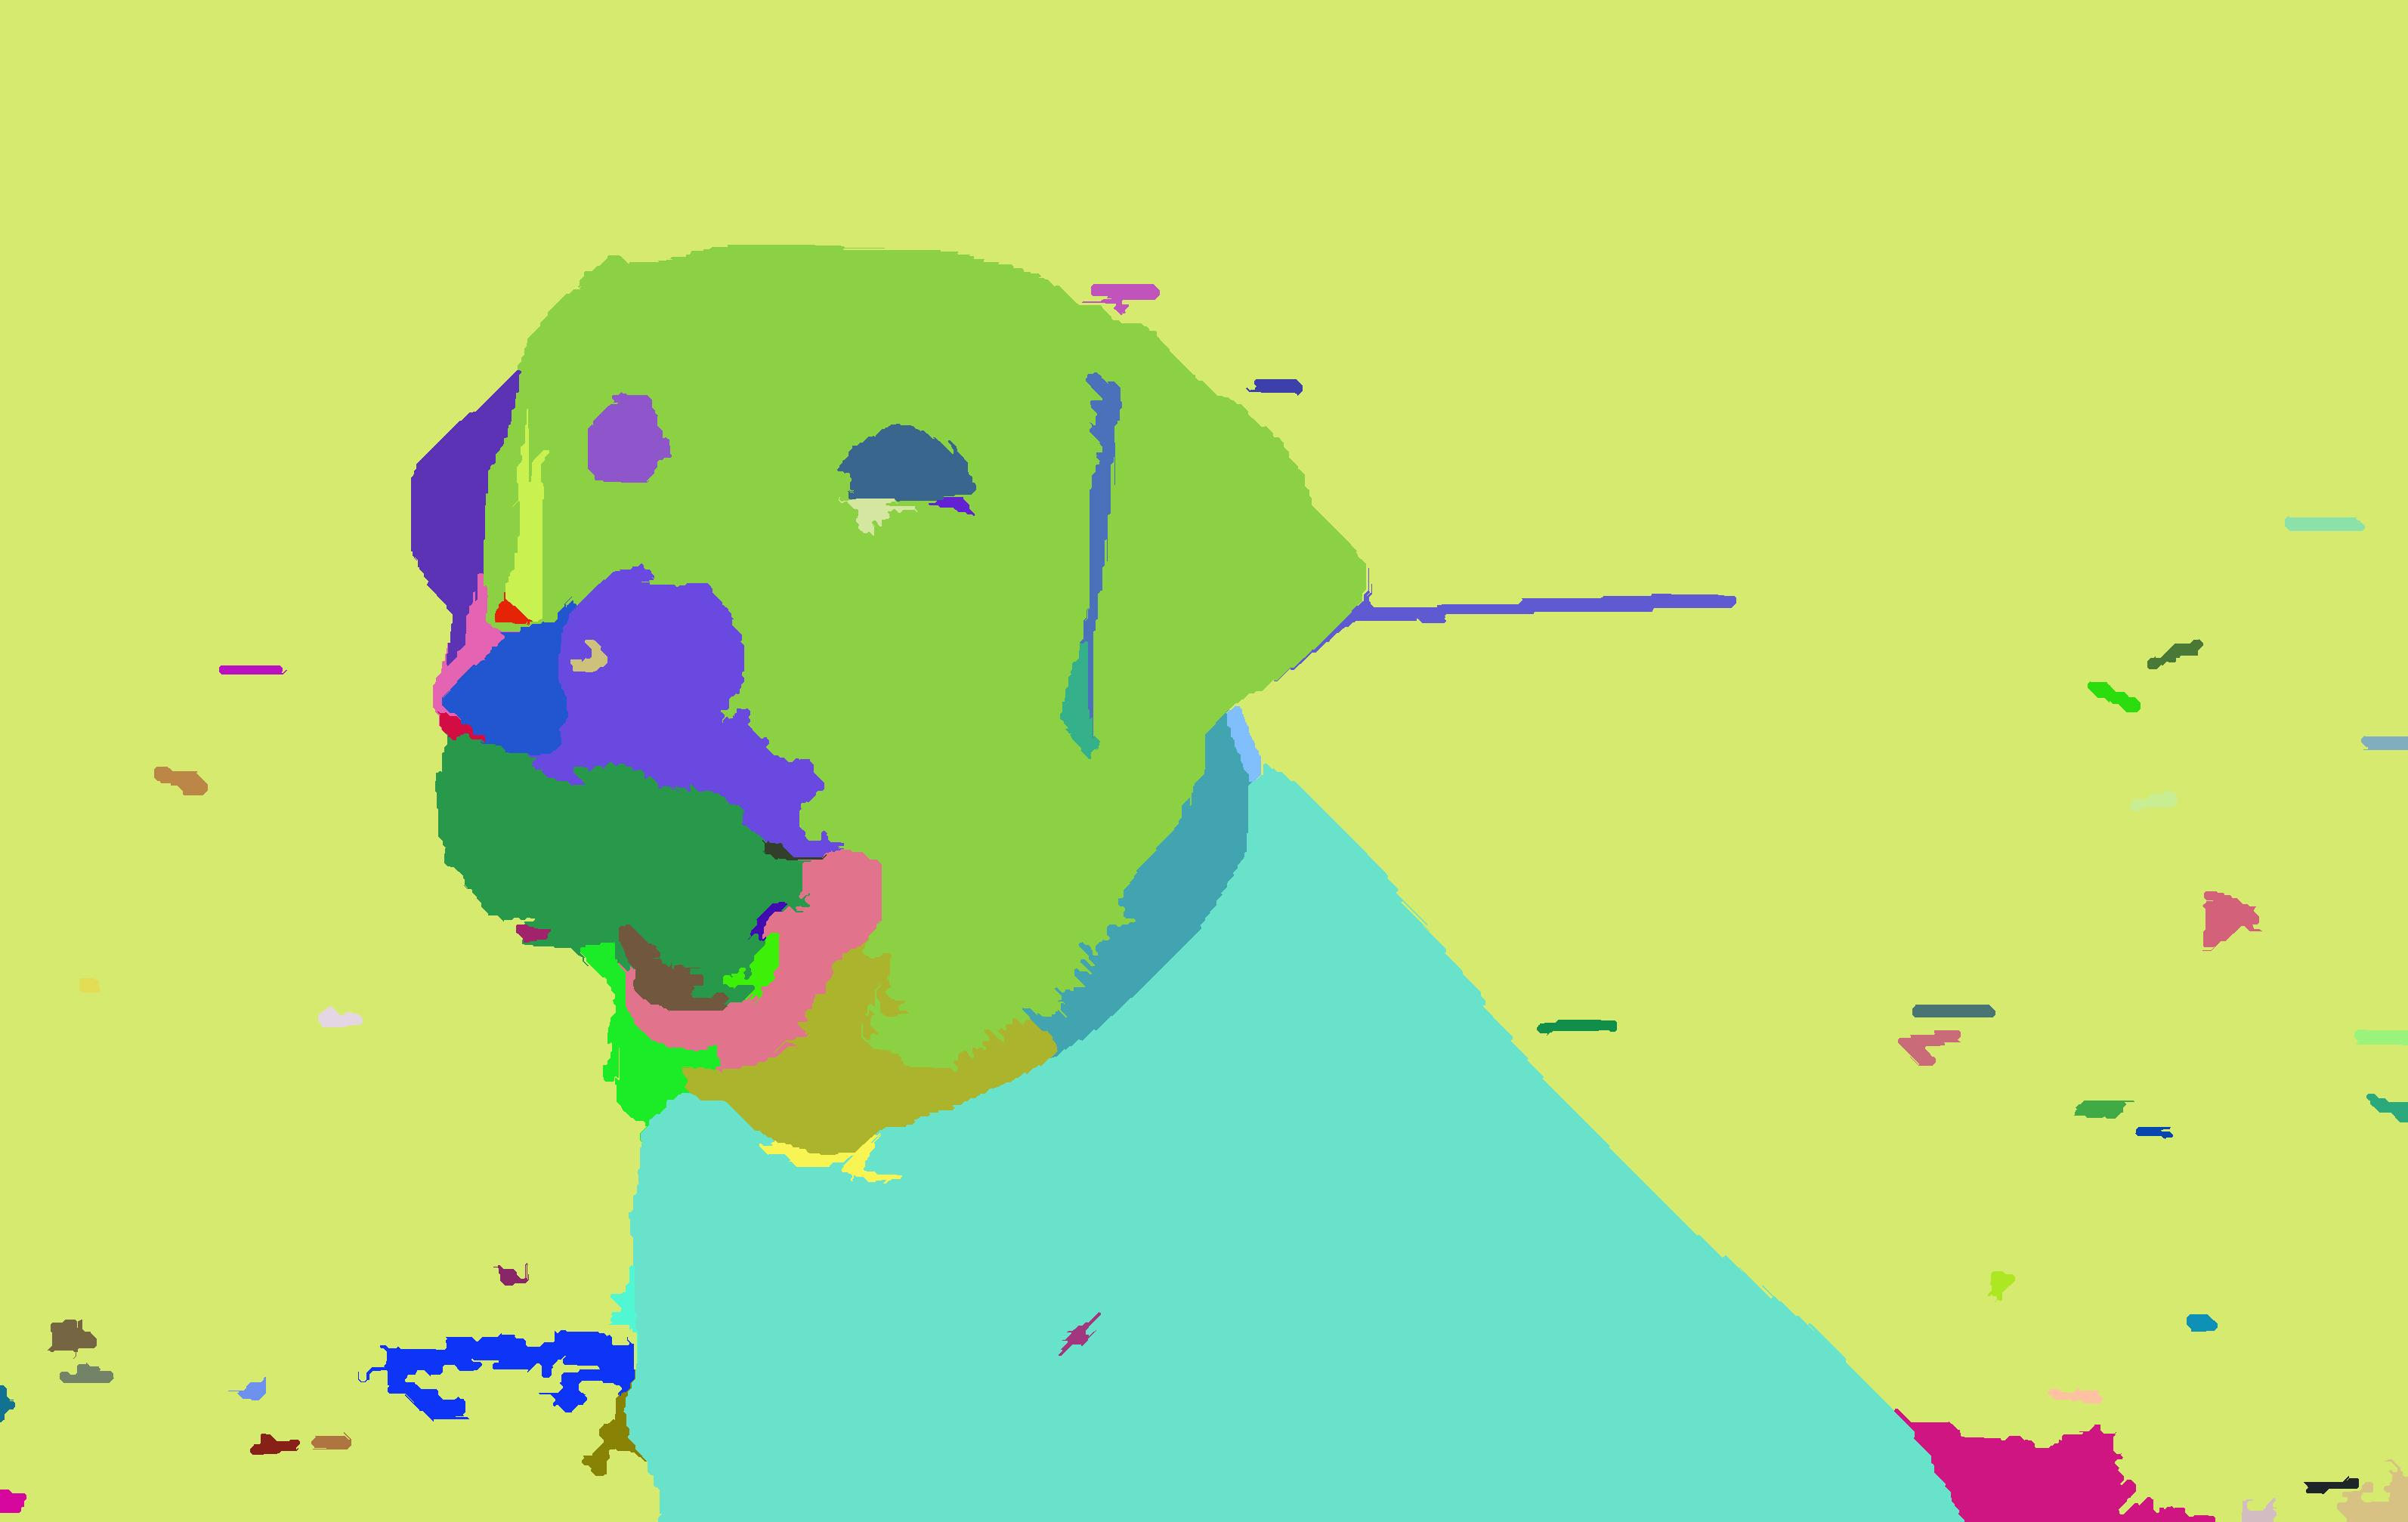
\includegraphics[width=\textwidth]{./img/our_dog.jpg}
                \caption{Dog picture segmented with our code}
                \label{ourdg}
        \end{subfigure}
        \begin{subfigure}[b]{0.3\textwidth}
                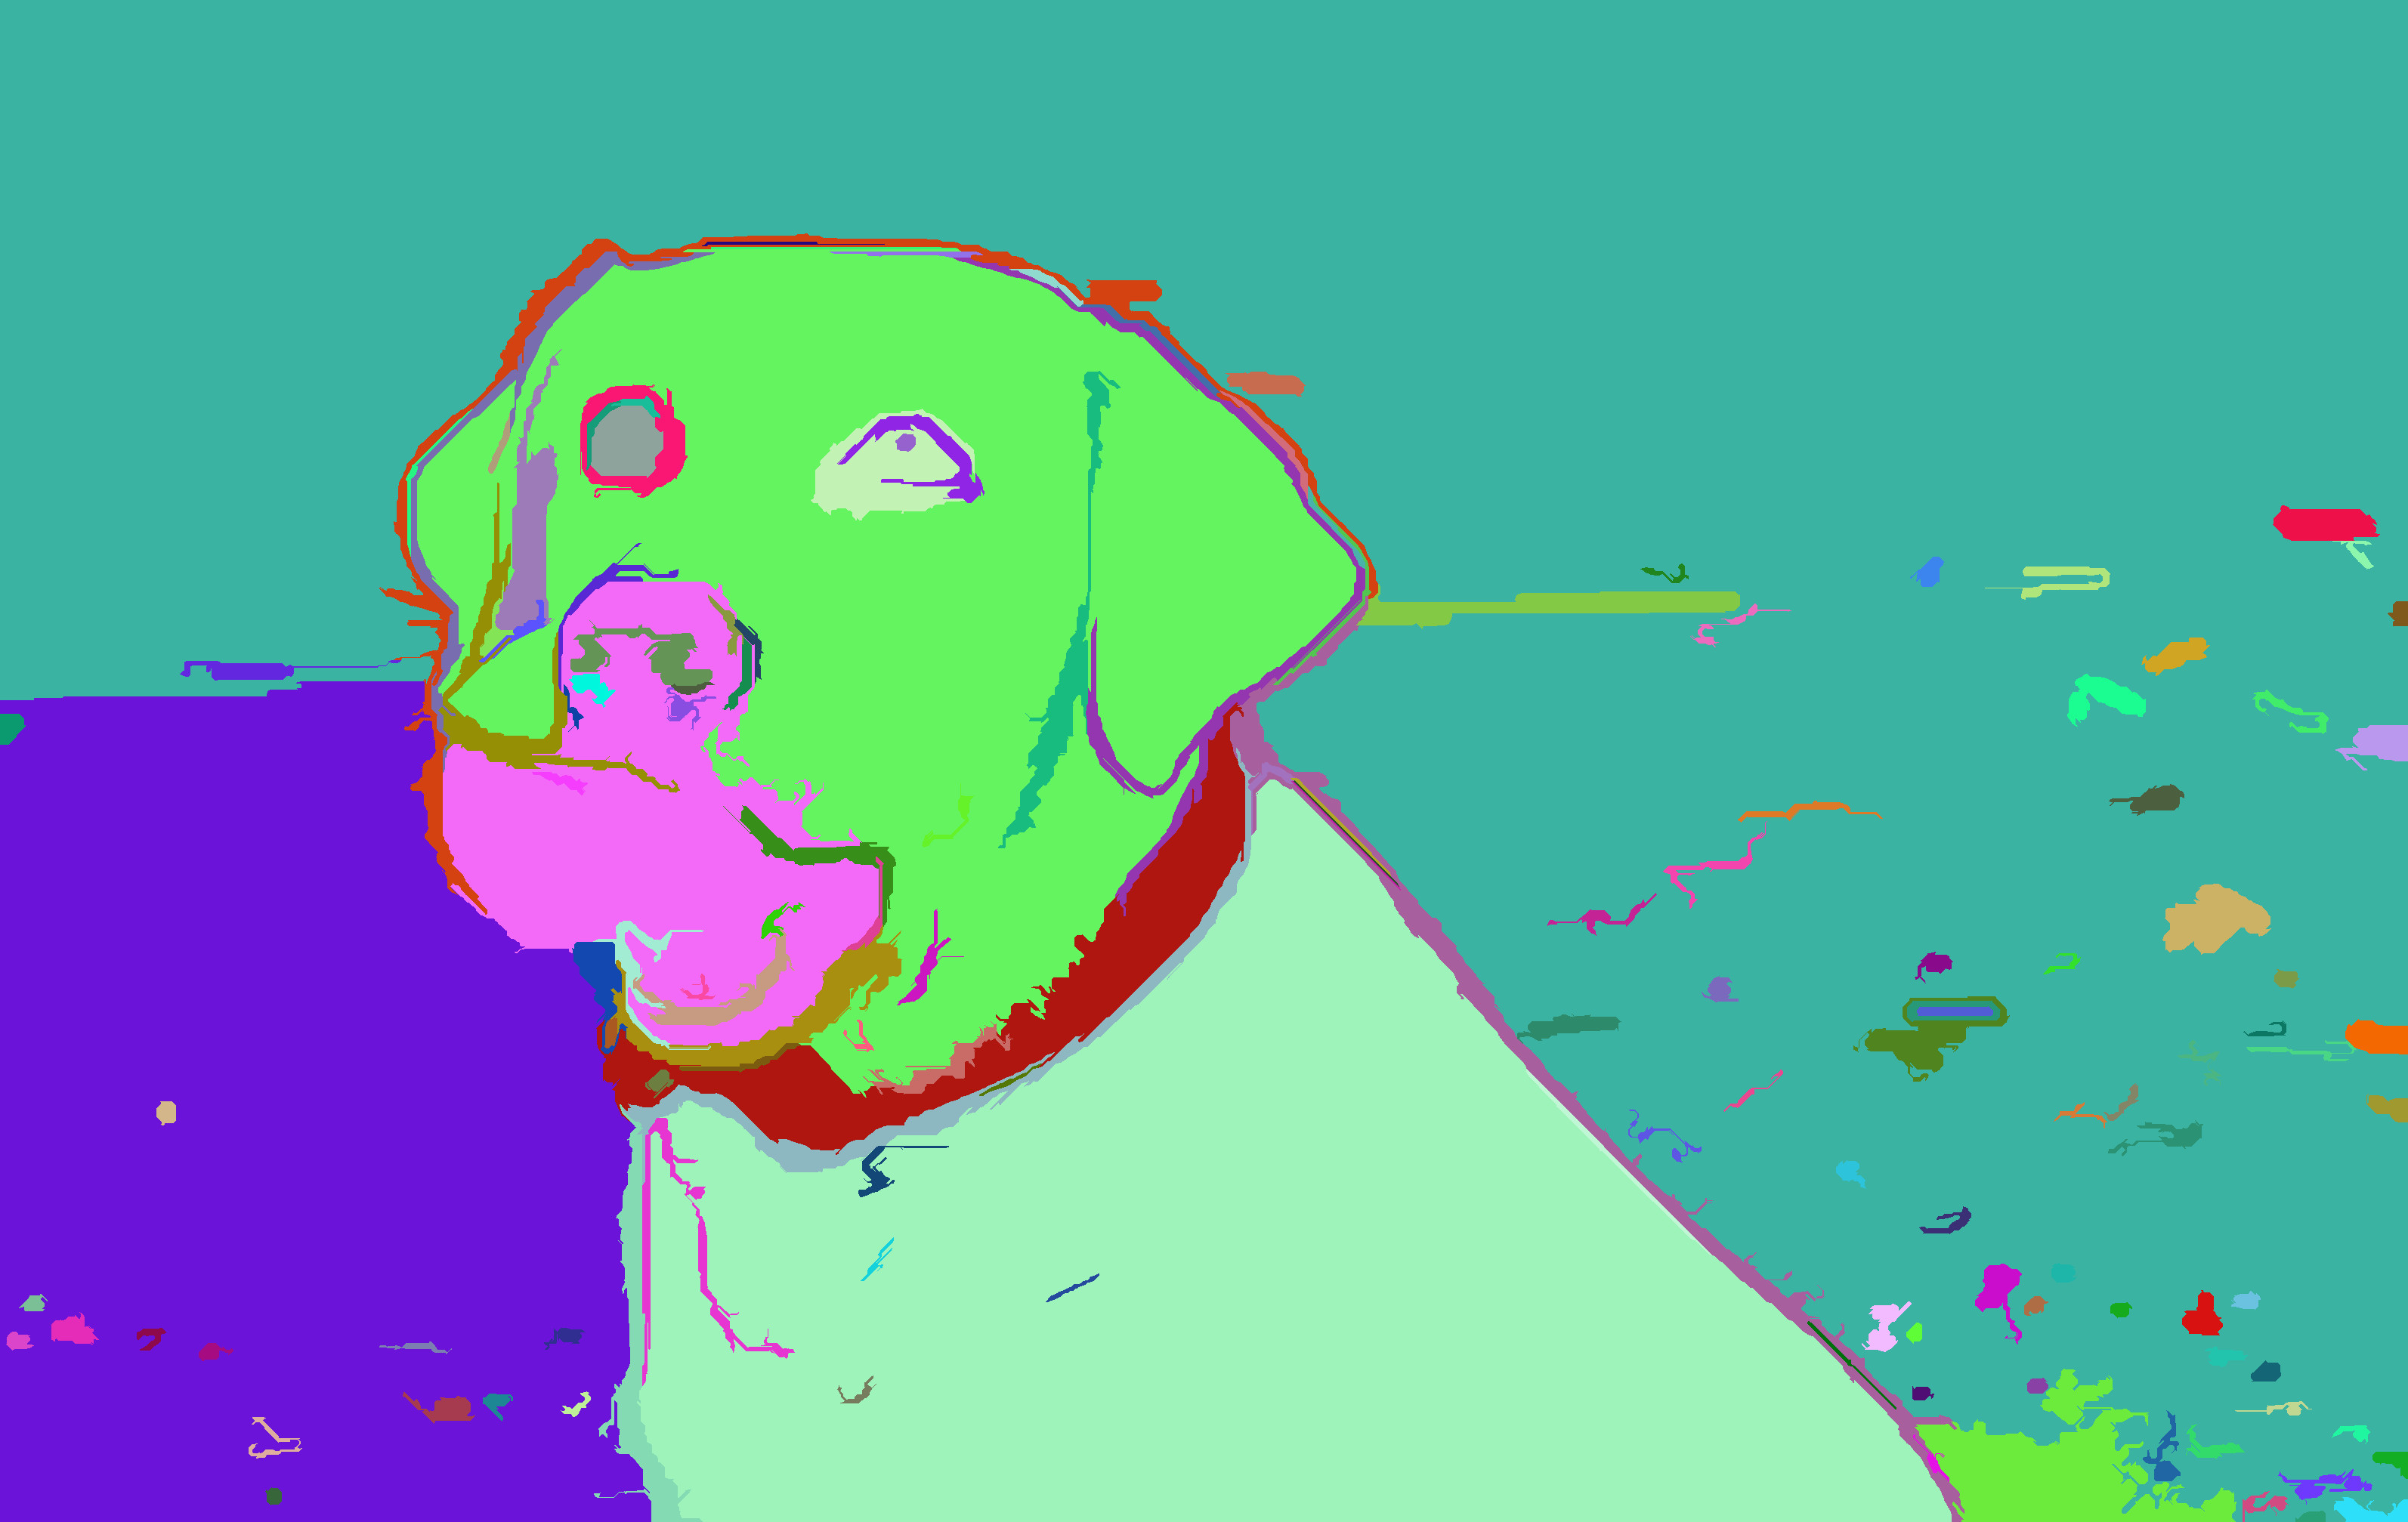
\includegraphics[width=\textwidth]{./img/their_dog.jpg}
                \caption{Dog picture segmented with author's code}
                \label{theirdg}
        \end{subfigure}
\end{figure}

Since one of the paper's main objectives is to collect noisy regions into components to account for textures, we believe our minimum size pre-condition is an improvement. The benchmark provides a quantitative backing for this assertion. Figures \ref{ogdog}, \ref{ourdg}, \ref{theirdg} illustrate he differences in segmentation results that we obtain.

\subsection{Benchmark}

We use the F-measure to compute segmentation accuracy against ground truth images. Table \ref{bench} summarizes our results.

\begin{table}
\begin{tabular}{|p{3cm}|c|c|c|c|c|}
\hline 
($\sigma$ = 4, minSize = 100, $K$ = 200) & Mailbox & Hand holding red berries & Moth & Frog & Frog with $\sigma=1$\tabularnewline
\hline 
\hline 
Our code & 0.9057 & 0.8242 & 0.9501 & 0.7842 & 0.8302\tabularnewline
\hline 
Author's code & 0.8365 & 0.8141 & 0.8520 & 0.3004 & 0.8208\tabularnewline
\hline
\end{tabular}
\caption{F-measure for Ground truth images}
\label{bench}
\end{table}

\subsection{Android App}

We implement an Android App that can take a picture from the camera and segment that image. We use OpenCV to convert the Bitmap format coming from the android camera to the Mat format which we can use to do a 2D Gaussian blur. We use the Android NDK toolkit to interface the core C++ segmentation function with Java to optimize performance. Functions building the connected graph and assigning the RGB color to disjoint sets are less critical, so we rewrite them in Java.

To illustrate the usage of our Android program, figure \ref{og} shows a picture taken from a phone and figure \ref{ogs} shows the segmented version of that image using our app. The segmentation process on the phone runs in a few seconds.

\begin{figure}
        \centering
        \begin{subfigure}[b]{0.3\textwidth}
                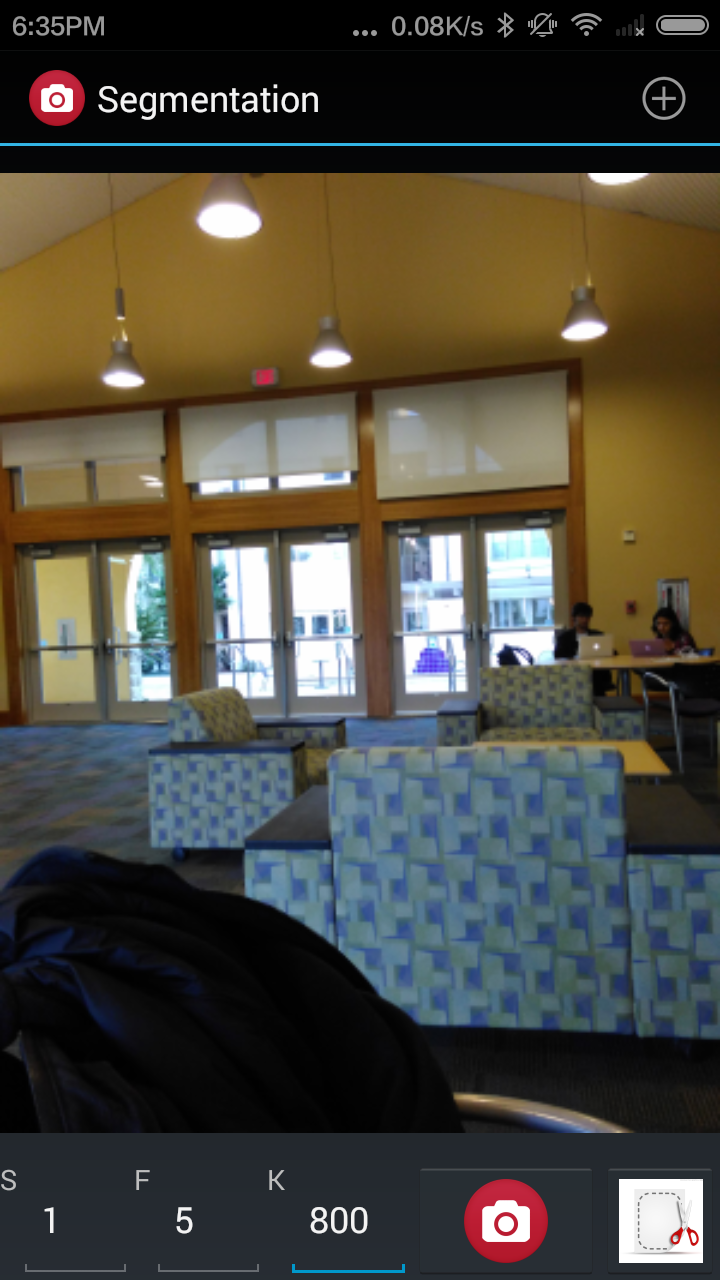
\includegraphics[width=\textwidth]{./img/screensh.png}
                \caption{Original image from Android phone}
                \label{og}
        \end{subfigure}
        \begin{subfigure}[b]{0.3\textwidth}
                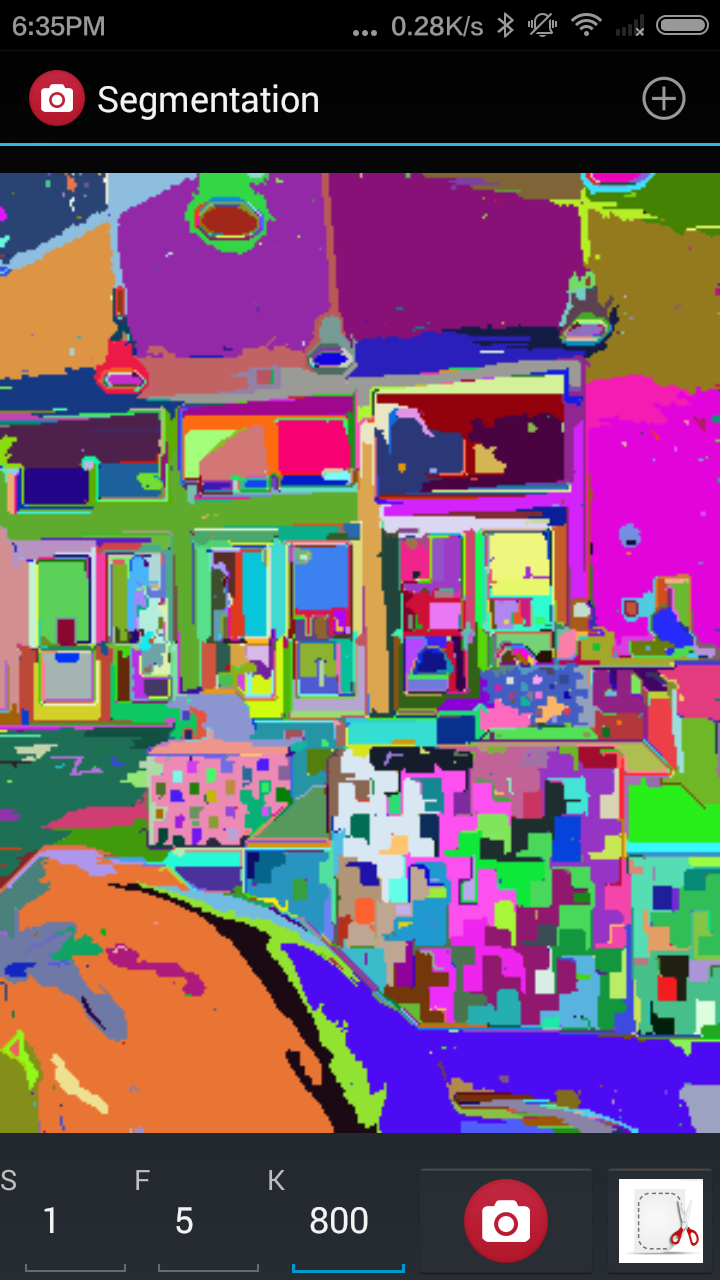
\includegraphics[width=\textwidth]{./img/screenshSEG.png}
                \caption{Segmented image from Android phone}
                \label{ogs}
        \end{subfigure}
\end{figure}

\subsection{Multi-Dimensional Graph Construction}

In this section, we explain why and how we built the multi-demisional graph, and the corresponding result.

In the author's original segmentation method, the graph was built in a Von Neumann Neighborhood or Moore Neighborhood. The weight of the edges is defined as the L2 distance of in the RGB color space for a color image or intensity difference for a gray-scale image. Their paper describes a method for building the graph in a multi-dimensional space, but they do not implement it \cite{paper}.

For the multi-dimesional graph, we use a 5-D feature space to describe every pixel. The components are: $X$, $Y$, $C_1$, $C_2$, $C_3$. X and Y are corresponding pixel coordinates. $C_1$, $C_2$, and $C_3$ are three components of a certain color space (R, G, and B for RGB color space). We used this 5-D feature space hoping that by combining pixel location information with pixel color information, we can achieve better segmentation results.

In this graph construction, the pixel difference is measured by L2 distance in the 5-D space. Based on this difference measure, every pixel is connected to the K nearest other pixels and a graph is formed.

It is important to note that the distance of the 5-D feature points are also sensitive to the value range of each component. For pixel coordinates X and Y, they would be dependent on the image size. For color components, the value range depends on the actual color space being used. In order to make a fair comparison between different color spaces and to achieve invariance for different image sizes, we normalized coordinates and color components to range from 0 to 1.

\begin{thebibliography}{1}
\small

\bibitem{paper}
Felzenszwalb, P. F., \& Huttenlocher, D. P. (2004).
	\emph{Efficient graph-based image segmentation}.
	International Journal of Computer Vision, 59(2), 167-181.

\end{thebibliography}
\end{document}